
\chapter{Overview and Descriptive Statistics}

\section{Populations and Samples}

\subsection{Facts and Concepts}

\begin{description}
	\item[data] collections of facts
	\item[population] collections of objects
	\item[census] collecting desired information for all objects in the population
	\item[sample] subsets of the population
	\item[variable] any characteristic whose value may change from one object to another in the population
	\item[univariate dataset] observations on a single variable
	\item[bivariate dataset] observations on two variables
	\item[multivariate dataset] observations on more than two variables
\end{description}

\section{Pictorial and Tabular Methods in Descriptive Statistics}

\subsection{Facts and Concepts}

\begin{description}
	\item[number of classes in histogram] $\rm\approx \sqrt{number\ of\ observations}$
	\item[density] $\rm\frac{relative\ frequency\ of\ the\ class}{class\ width}$
	\item[relative frequency] $\rm\frac{number\ of\ times\ the\ value\ appers}{number\ of\ observations\ in\ the\ dataset}$
	\item[unimodal histogram] one that rises to a single peak and then declines
	\item[bimodal histogram] one that has two different peaks
	\item[multimodal histogram] one that has more than two peaks
	\item[symmetric] left half of graph is a mirror image of the right half
	\item[positively skewed] the right or upper tail is stretched out compared with the left or lower tail
	\item[negatively skewed] the left or lower tail is stretched out compared with the right or upper tail
\end{description}

\begin{figure}[H]
	\centering
	\small
	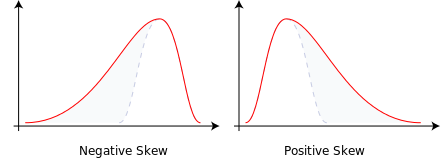
\includegraphics[width=0.8\textwidth]{img/1-negative-positive-skew}
	\caption{Negative and Positive Skew}
	\label{fig:1}
\end{figure}

\section{Measures of Location}

\subsection{Facts and Concepts}

\begin{description}
	\item[sample mean]
	$$\bar{x} = \frac{x_1 + x_2 + \dots + x_n}{n} = \frac{\sum\limits_{i= 1}^{n} x_i}{n}$$
	\item[sample median]
	$$\tilde{x} = 
	\left\{\begin{array}{ll}
	{\rm The\ single\ middle\ value\ if\ }n{\rm\ is\ odd} &
	= \left( \frac{n + 1}{2} \right) ^ {\rm th} {\rm ordered\ value}\\
	{\rm The\ average\ of\ the\ two\ middle\ values\ if\ }n{\rm \ is\ even} &
	= {\rm average\ of\ } \left( \frac{n}{2} \right) ^ {\rm th} {\rm \ and\ }\left( \frac{n}{2} + 1 \right) ^ {\rm th} {\rm \ ordered\ values} \\
	\end{array}\right.$$
	\item[population mean and population median] $\mu$ and $\tilde{\mu}$\\
	Negative skew if $\mu < \tilde{\mu}$;\\
	Symmetric if $\mu = \tilde{\mu}$;\\
	Positive skew if $\mu > \tilde{\mu}$;
	\item[n\% trimmed mean] average of samples without the smallest $n$\% and the largest $n$\%
	\item[n\% percentile] samples without the highest $n$\%
\end{description}

\section{Measures of Variability}

\subsection{Facts and Concepts}

\begin{description}
	\item[sample variance]
	$$ s ^ 2 = \frac{\sum \left(x_i - \bar{x}\right) ^ 2}{n - 1} = \frac{S_{xx}}{n - 1}$$\\
	\rule{\linewidth}{1pt}
	\par An alternative expression for the numerator of $s ^ 2$ is
	$$S_{xx} = \sum \left( x_i - \bar{x} \right) ^ 2 = \sum x_i ^ 2 - \frac{\left( \sum x_i \right) ^ 2}{n} $$
	\begin{proof}
		Because
		
		$$\bar{x} = \frac{\sum x_i}{n},\ n\bar{x} ^ 2= \frac{n\left( \sum x_i \right) ^ 2}{n ^ 2} = \frac{\left( \sum x_i \right) ^ 2}{n} $$
		
		then
		\begin{align*}
		\sum\left( x_i - \bar{x} \right) ^ 2 &= \sum \left( x_i ^ 2 - 2 \bar{x}\cdot x + \bar{x} ^ 2\right) = \sum x_i ^ 2 - 2 \bar{x}\sum x_i + \sum \left( \bar{x} ^ 2 \right) \\
		&= \sum x_i ^ 2 - 2 \bar{x} \cdot n \bar{x} + n \left( \bar{x} \right) ^ 2 = \sum x_i ^ 2 - n \left( \bar{x} \right) ^ 2 = \sum x_i ^ 2 - \frac{\left( \sum x_i\right) ^ 2}{n} \tag*{\qedhere}\\
		\end{align*}
	\end{proof}
	\rule{\linewidth}{1pt}
	\item[sample standard deviation]
	$$ s = \sqrt{s ^ 2} $$
	\item[population variance]
	$$ \sigma ^ 2 = \frac{\sum\limits_{i = 1} ^ {N} \left( x_i - \mu \right) ^2}{N} $$
	\item[population standard deviation]
	$$ \sigma = \sqrt{\sigma ^ 2} $$
	\item[fourth spread]
	$$f_s={\rm upper\ fourth} - {\rm lower\ fourth}$$
	where observations are ordered and separated in half(median in both halves if odd number) and upper fourth is median in the larger half, lower fourth is median in the smaller half\\
	\rule{\linewidth}{1pt}
	\par Any observation farther than $1.5f_s$ from the closest fourth is an \textbf{outlier}. An outlier is \textbf{extreme} if it is more than $3f_s$ from the nearest fourth, and it is \textbf{mild} otherwise.\\
	\rule{\linewidth}{1pt}
\end{description}
